\documentclass[xetex]{beamer}

\usepackage[english]{babel}
\usepackage{polyglossia}
\setdefaultlanguage{french}
\usepackage{graphicx}
\usepackage{adjustbox}
\usepackage{tikz, pgfplots}
\usetheme{modern}


\title
    {Architecture des systèmes d'information}
\subtitle
    {Gestion des contacts d'une banque}
\author
    {H4401}


\begin{document}

    \frame[plain]{\titlepage}

    \frame{\tableofcontents}

    \section{Découpage MCD et objets métier (Antoine)}
     \begin{frame}{Découpage MCD (1)}
	
\noindent\makebox[\textwidth]{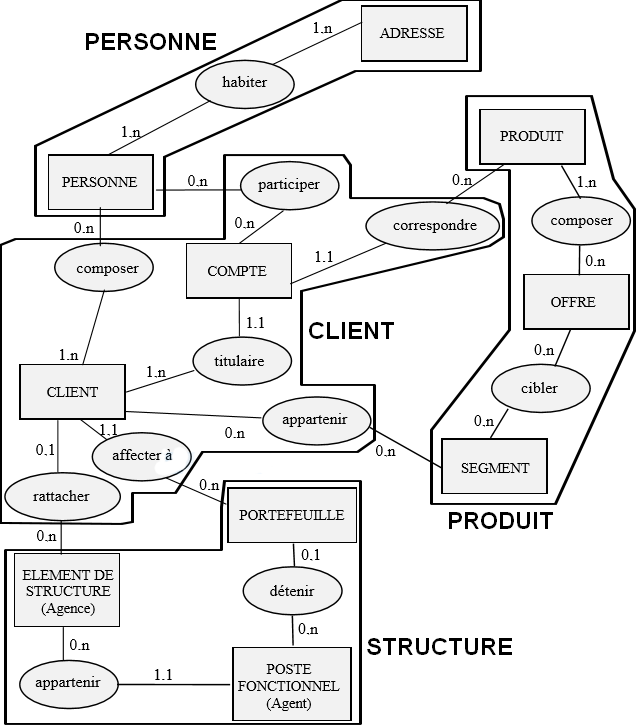
\includegraphics[height=8cm]{../report/figures/mcd/MCD_Clients_Produits.png}}

    \end{frame}
    \begin{frame}{Découpage MCD (2)}
\noindent\makebox[\textwidth]{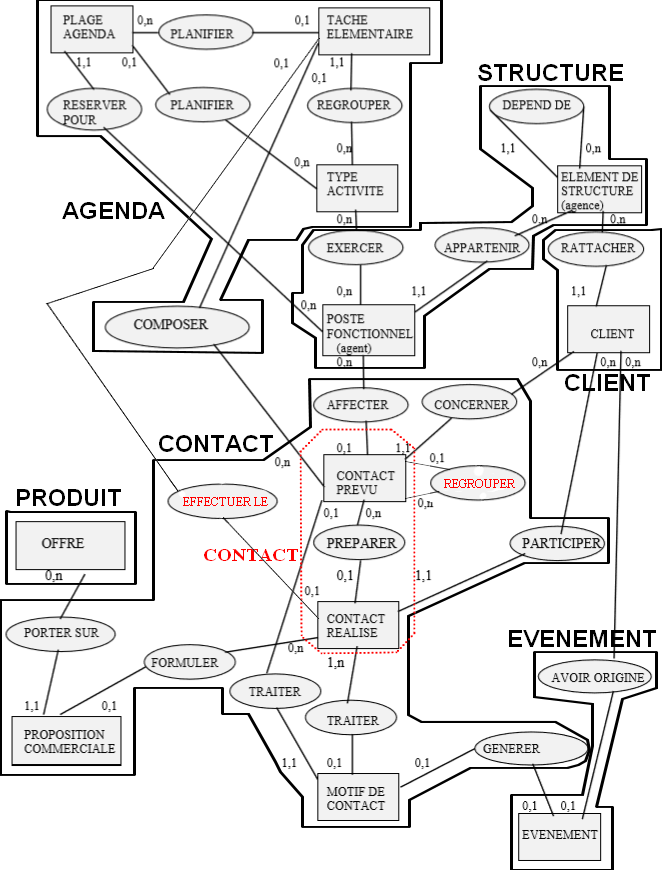
\includegraphics[height=8cm]{../report/figures/mcd/MCD_Commercial.png}}
    \end{frame}
    \section{Diagramme d’état (Paul)}
    \begin{frame}{Diagramme d'état de l'objet contact}
\noindent\makebox[\textwidth]{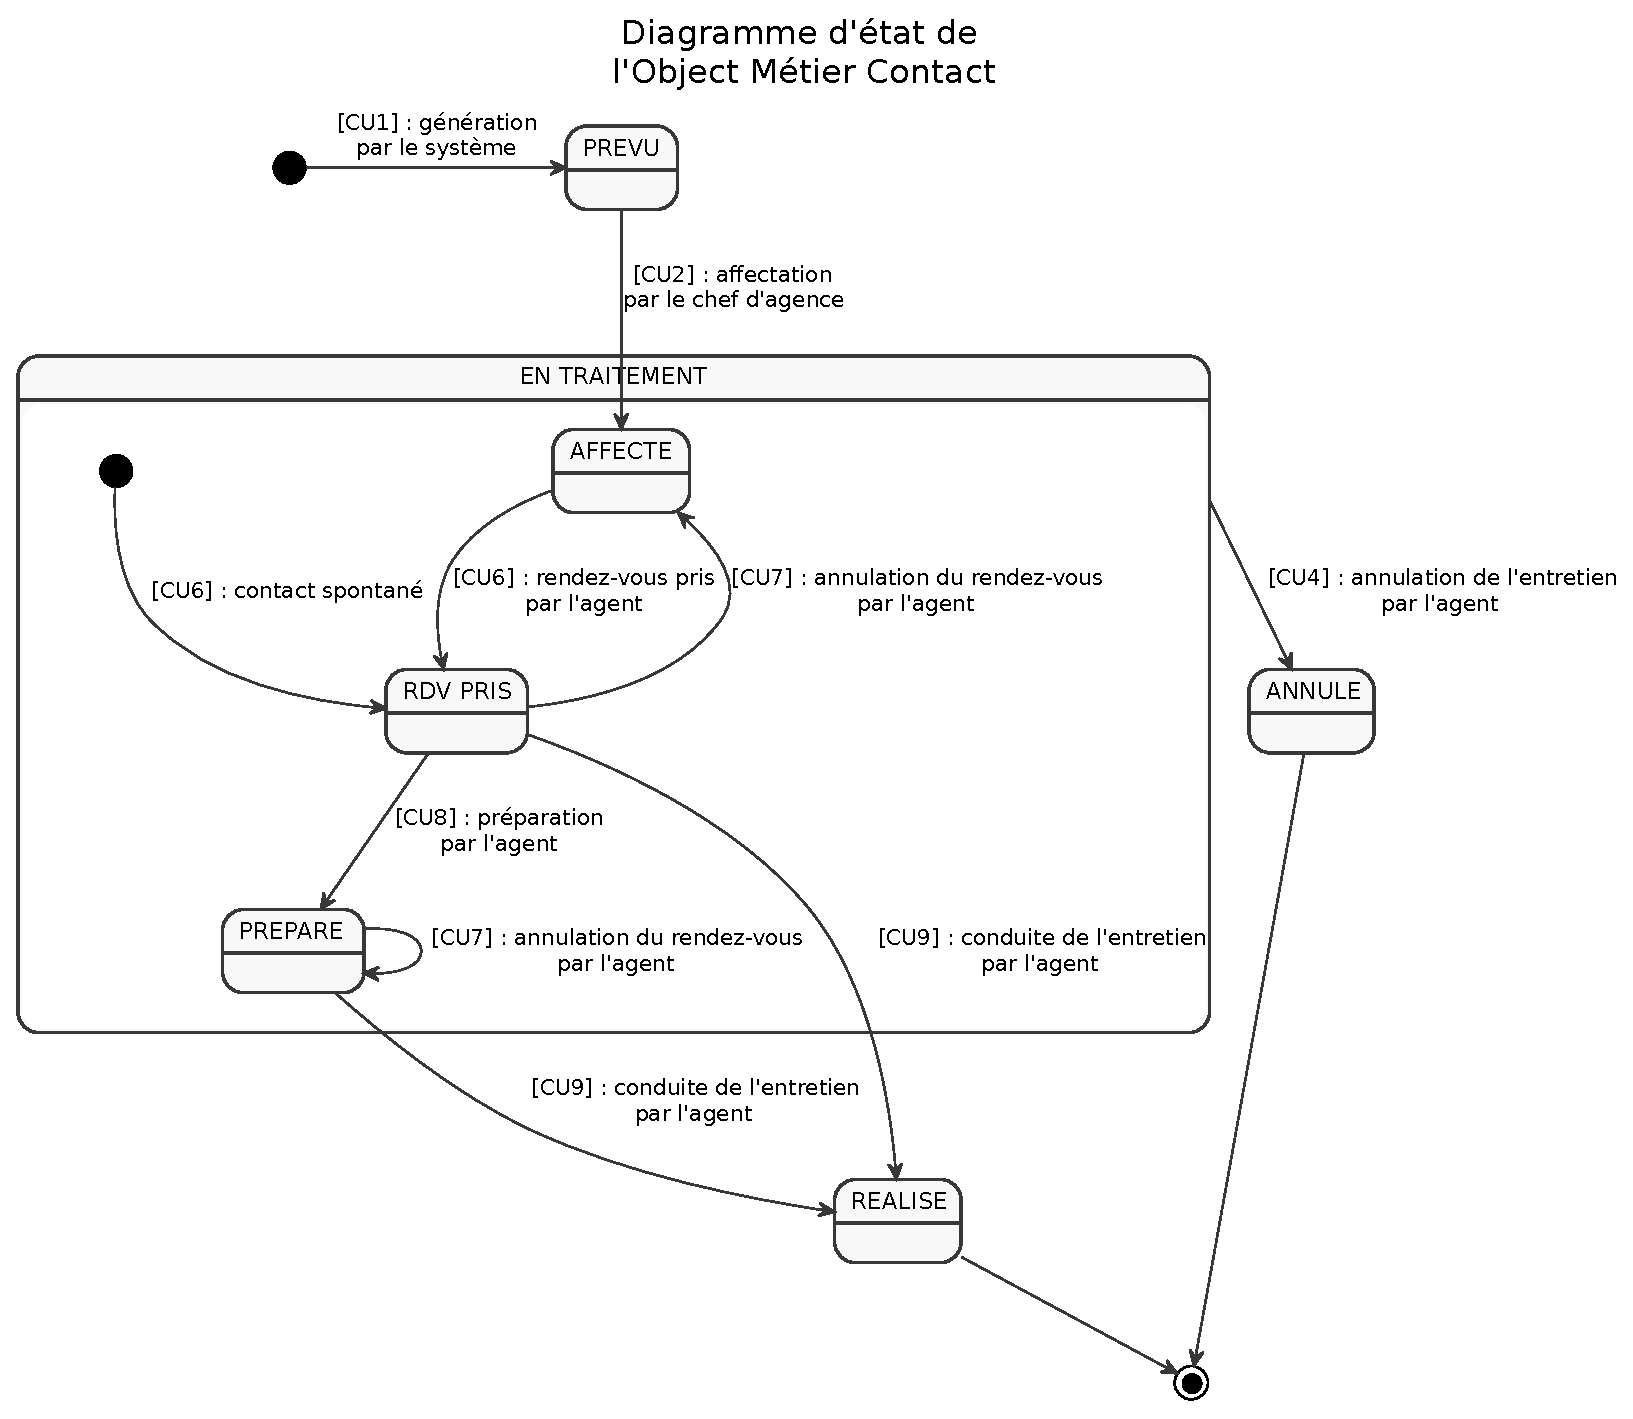
\includegraphics[height=8cm]{../report/figures/eps/diag_etats_contact}}
    \end{frame}
    \section{IHM Agenda (Hugues)}

 \begingroup
        \setbeamercolor{background canvas}{parent=palette secondary}
        \begin{frame}[plain]
            \centering
            \vfill
            \usebeamerfont{section title}\usebeamercolor[fg]{frametitle}IHM Agenda
            \vfill
        \end{frame}
    \endgroup    
    
    \section{Diagramme de séquence détaillé - CU7 (Lisa)}
    \begin{frame}{Diagramme de séquence détaillé - CU7}
    \adjustbox{width=1.1\textwidth, center, trim={0} {.45\height} {0} {0.15cm},clip}%
  {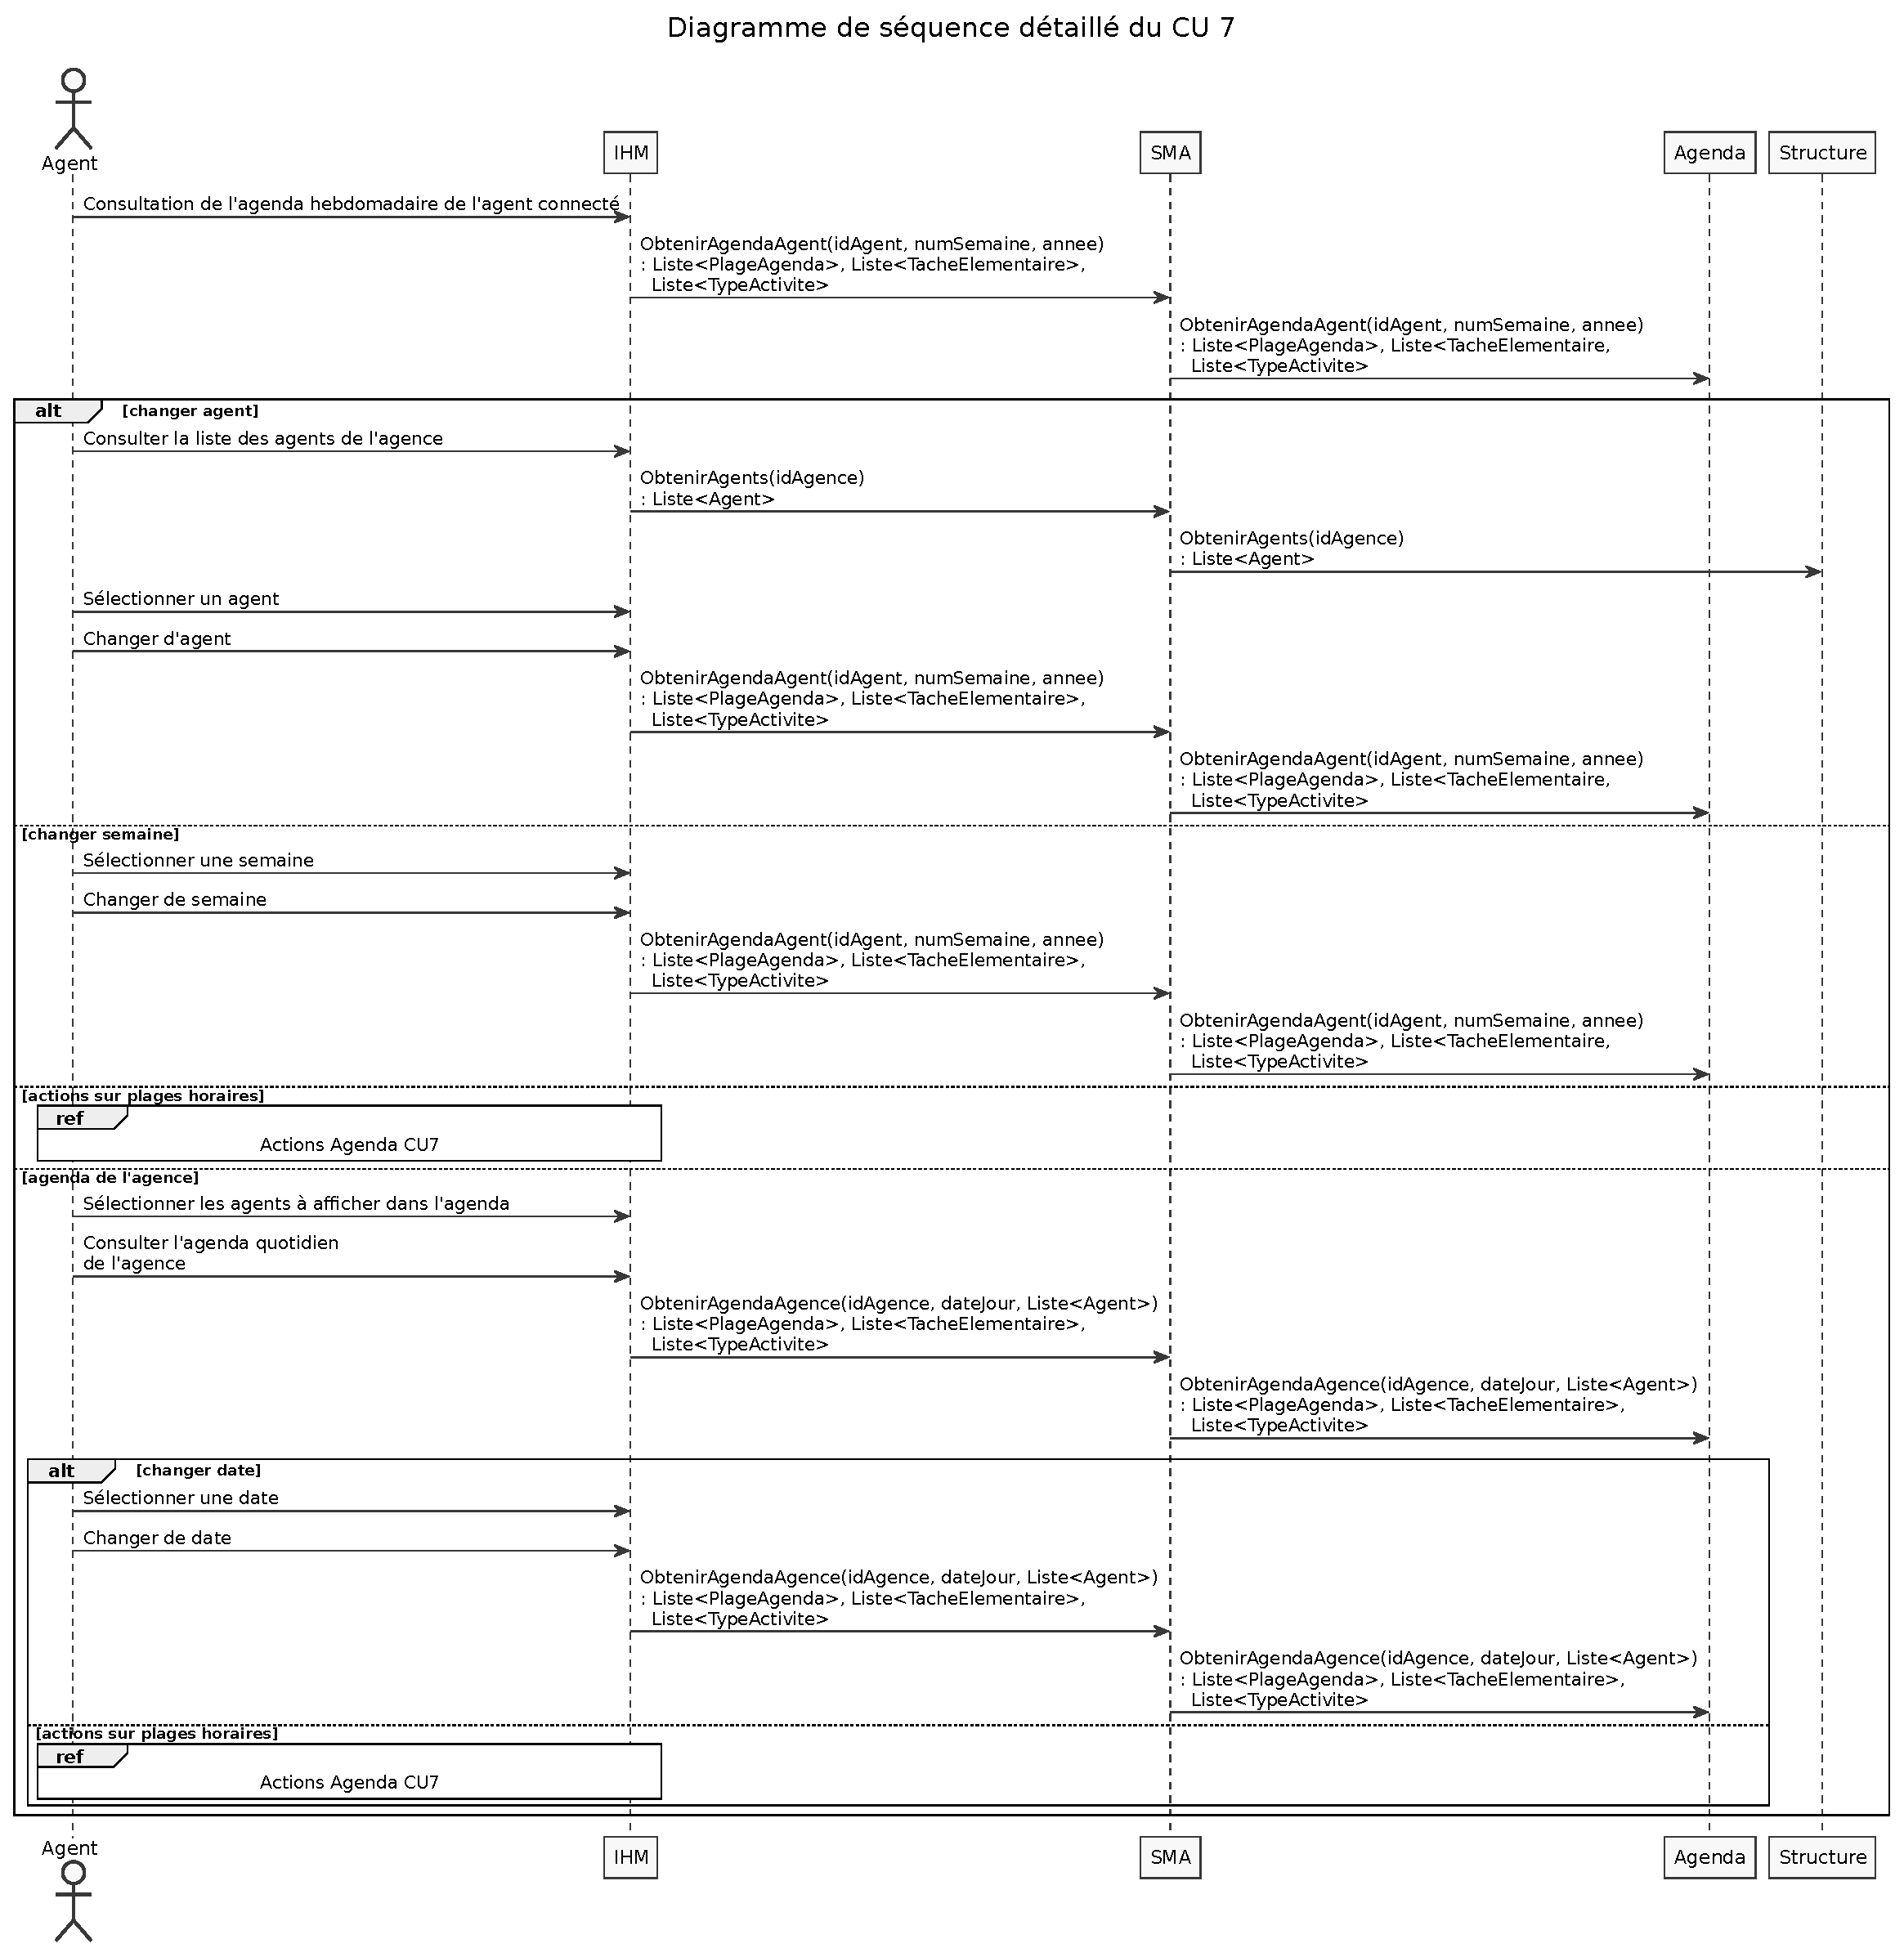
\includegraphics[height=12cm]{../report/figures/eps/DSD_CU7}}
    \end{frame}
    
    
        \begin{frame}{Diagramme de séquence détaillé - CU7}
    \adjustbox{width=1.1\textwidth, center, trim={0} {0} {0} {.55\height},clip}
  {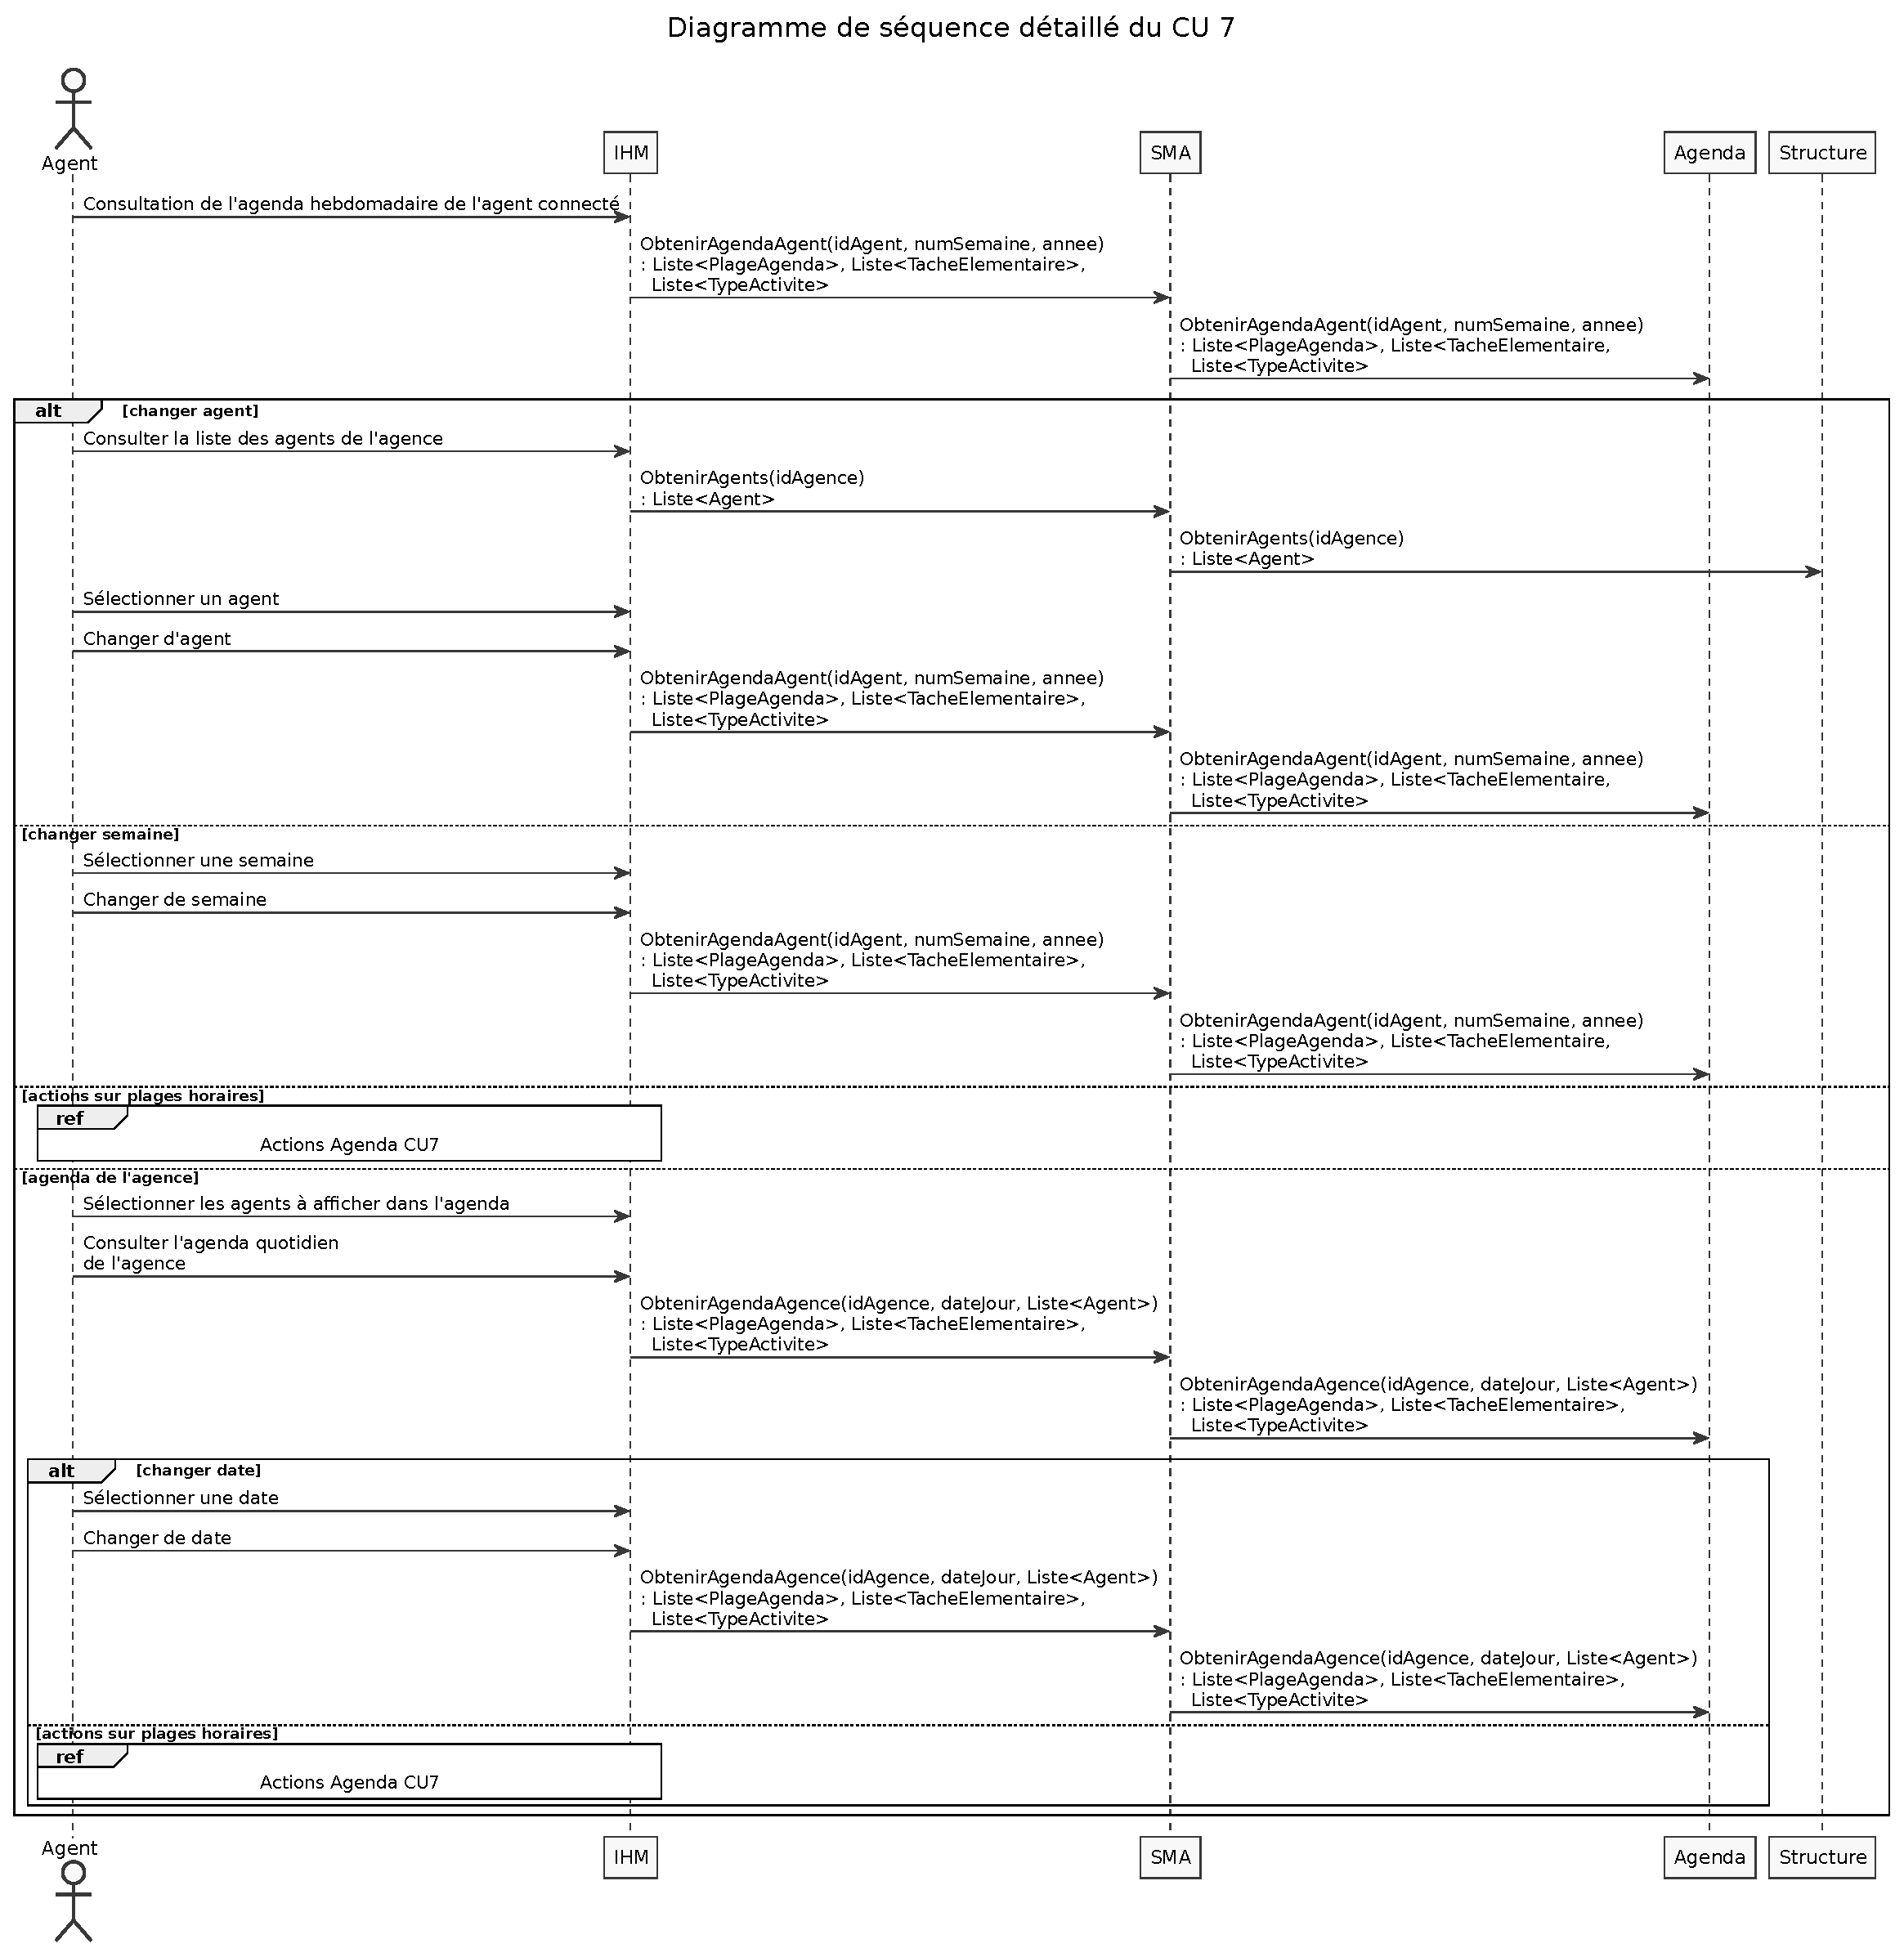
\includegraphics[height=12cm]{../report/figures/eps/DSD_CU7}}
    \end{frame}
    
    \begin{frame}{Diagramme de séquence détaillé - Action Agenda}
    
    \transwipe
\only<1>{    \adjustbox{width=1.1\textwidth, center, trim={0} {.5\height} {0} {0},clip}%
  {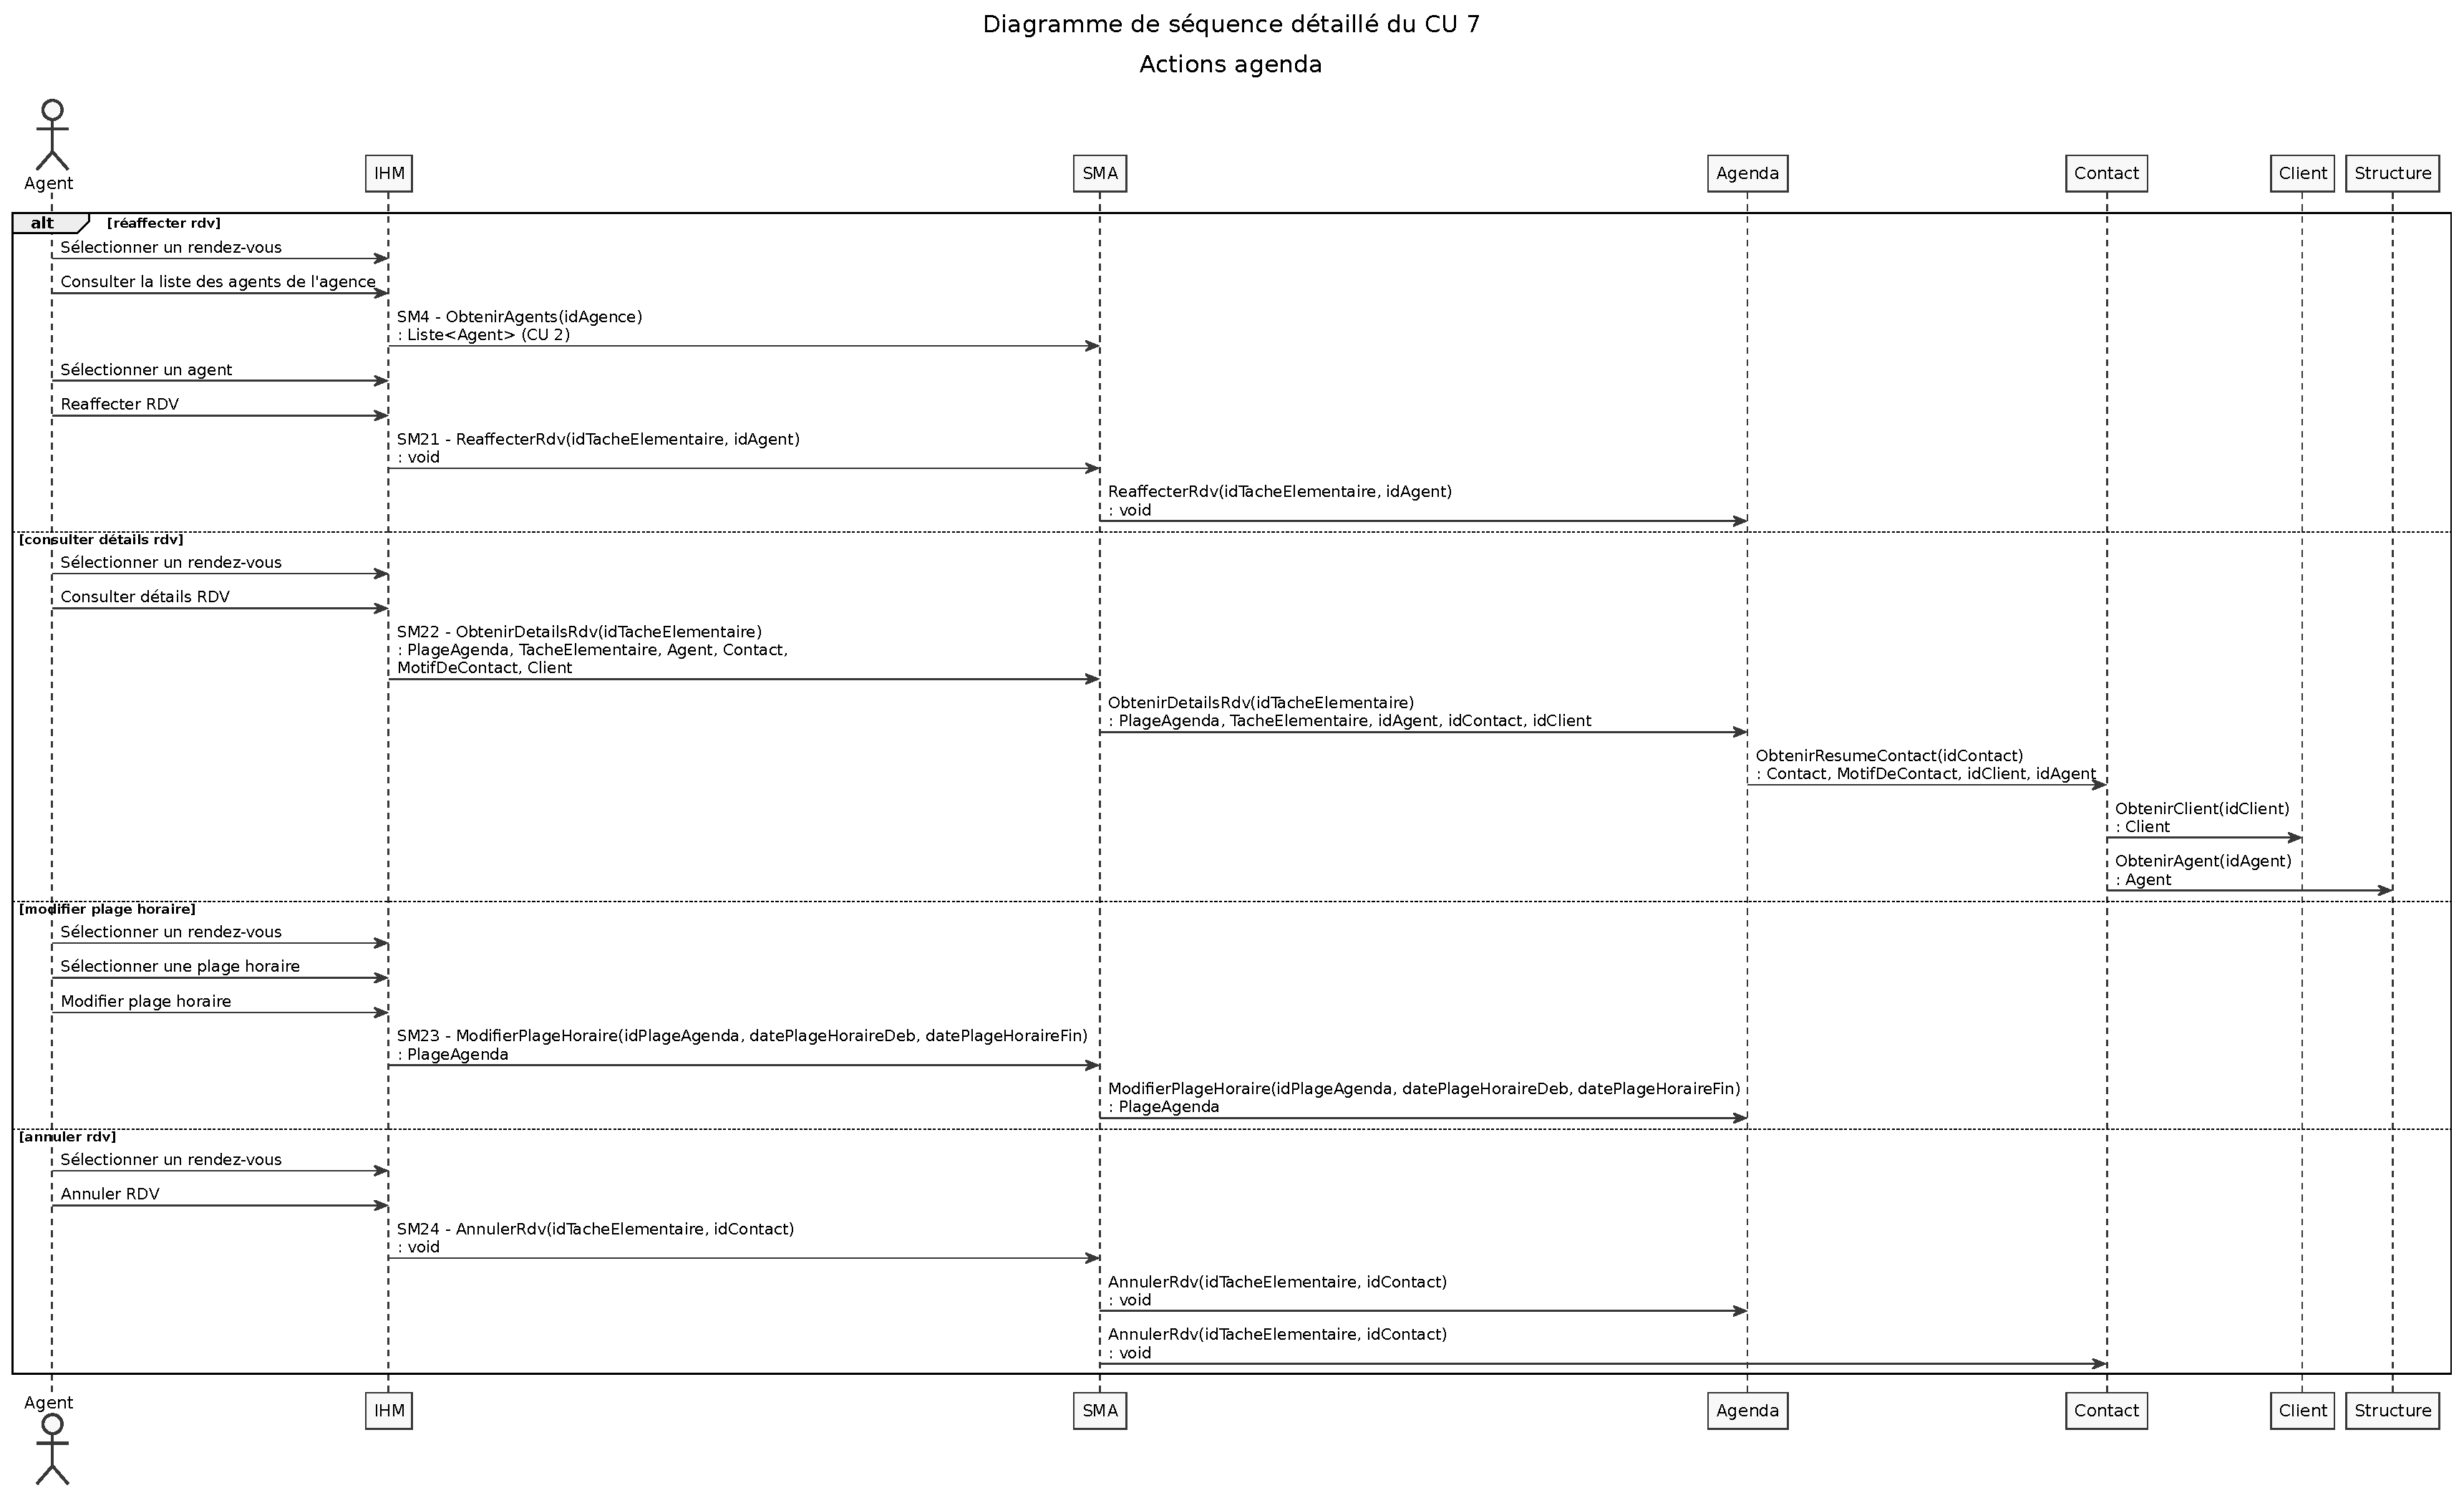
\includegraphics[height=12cm]{../report/figures/eps/DSD_CU7_ActionsAgenda}}}
\only<2>{\adjustbox{width=1.1\textwidth, center, trim={0} {0} {0} {.5\height},clip}%
  {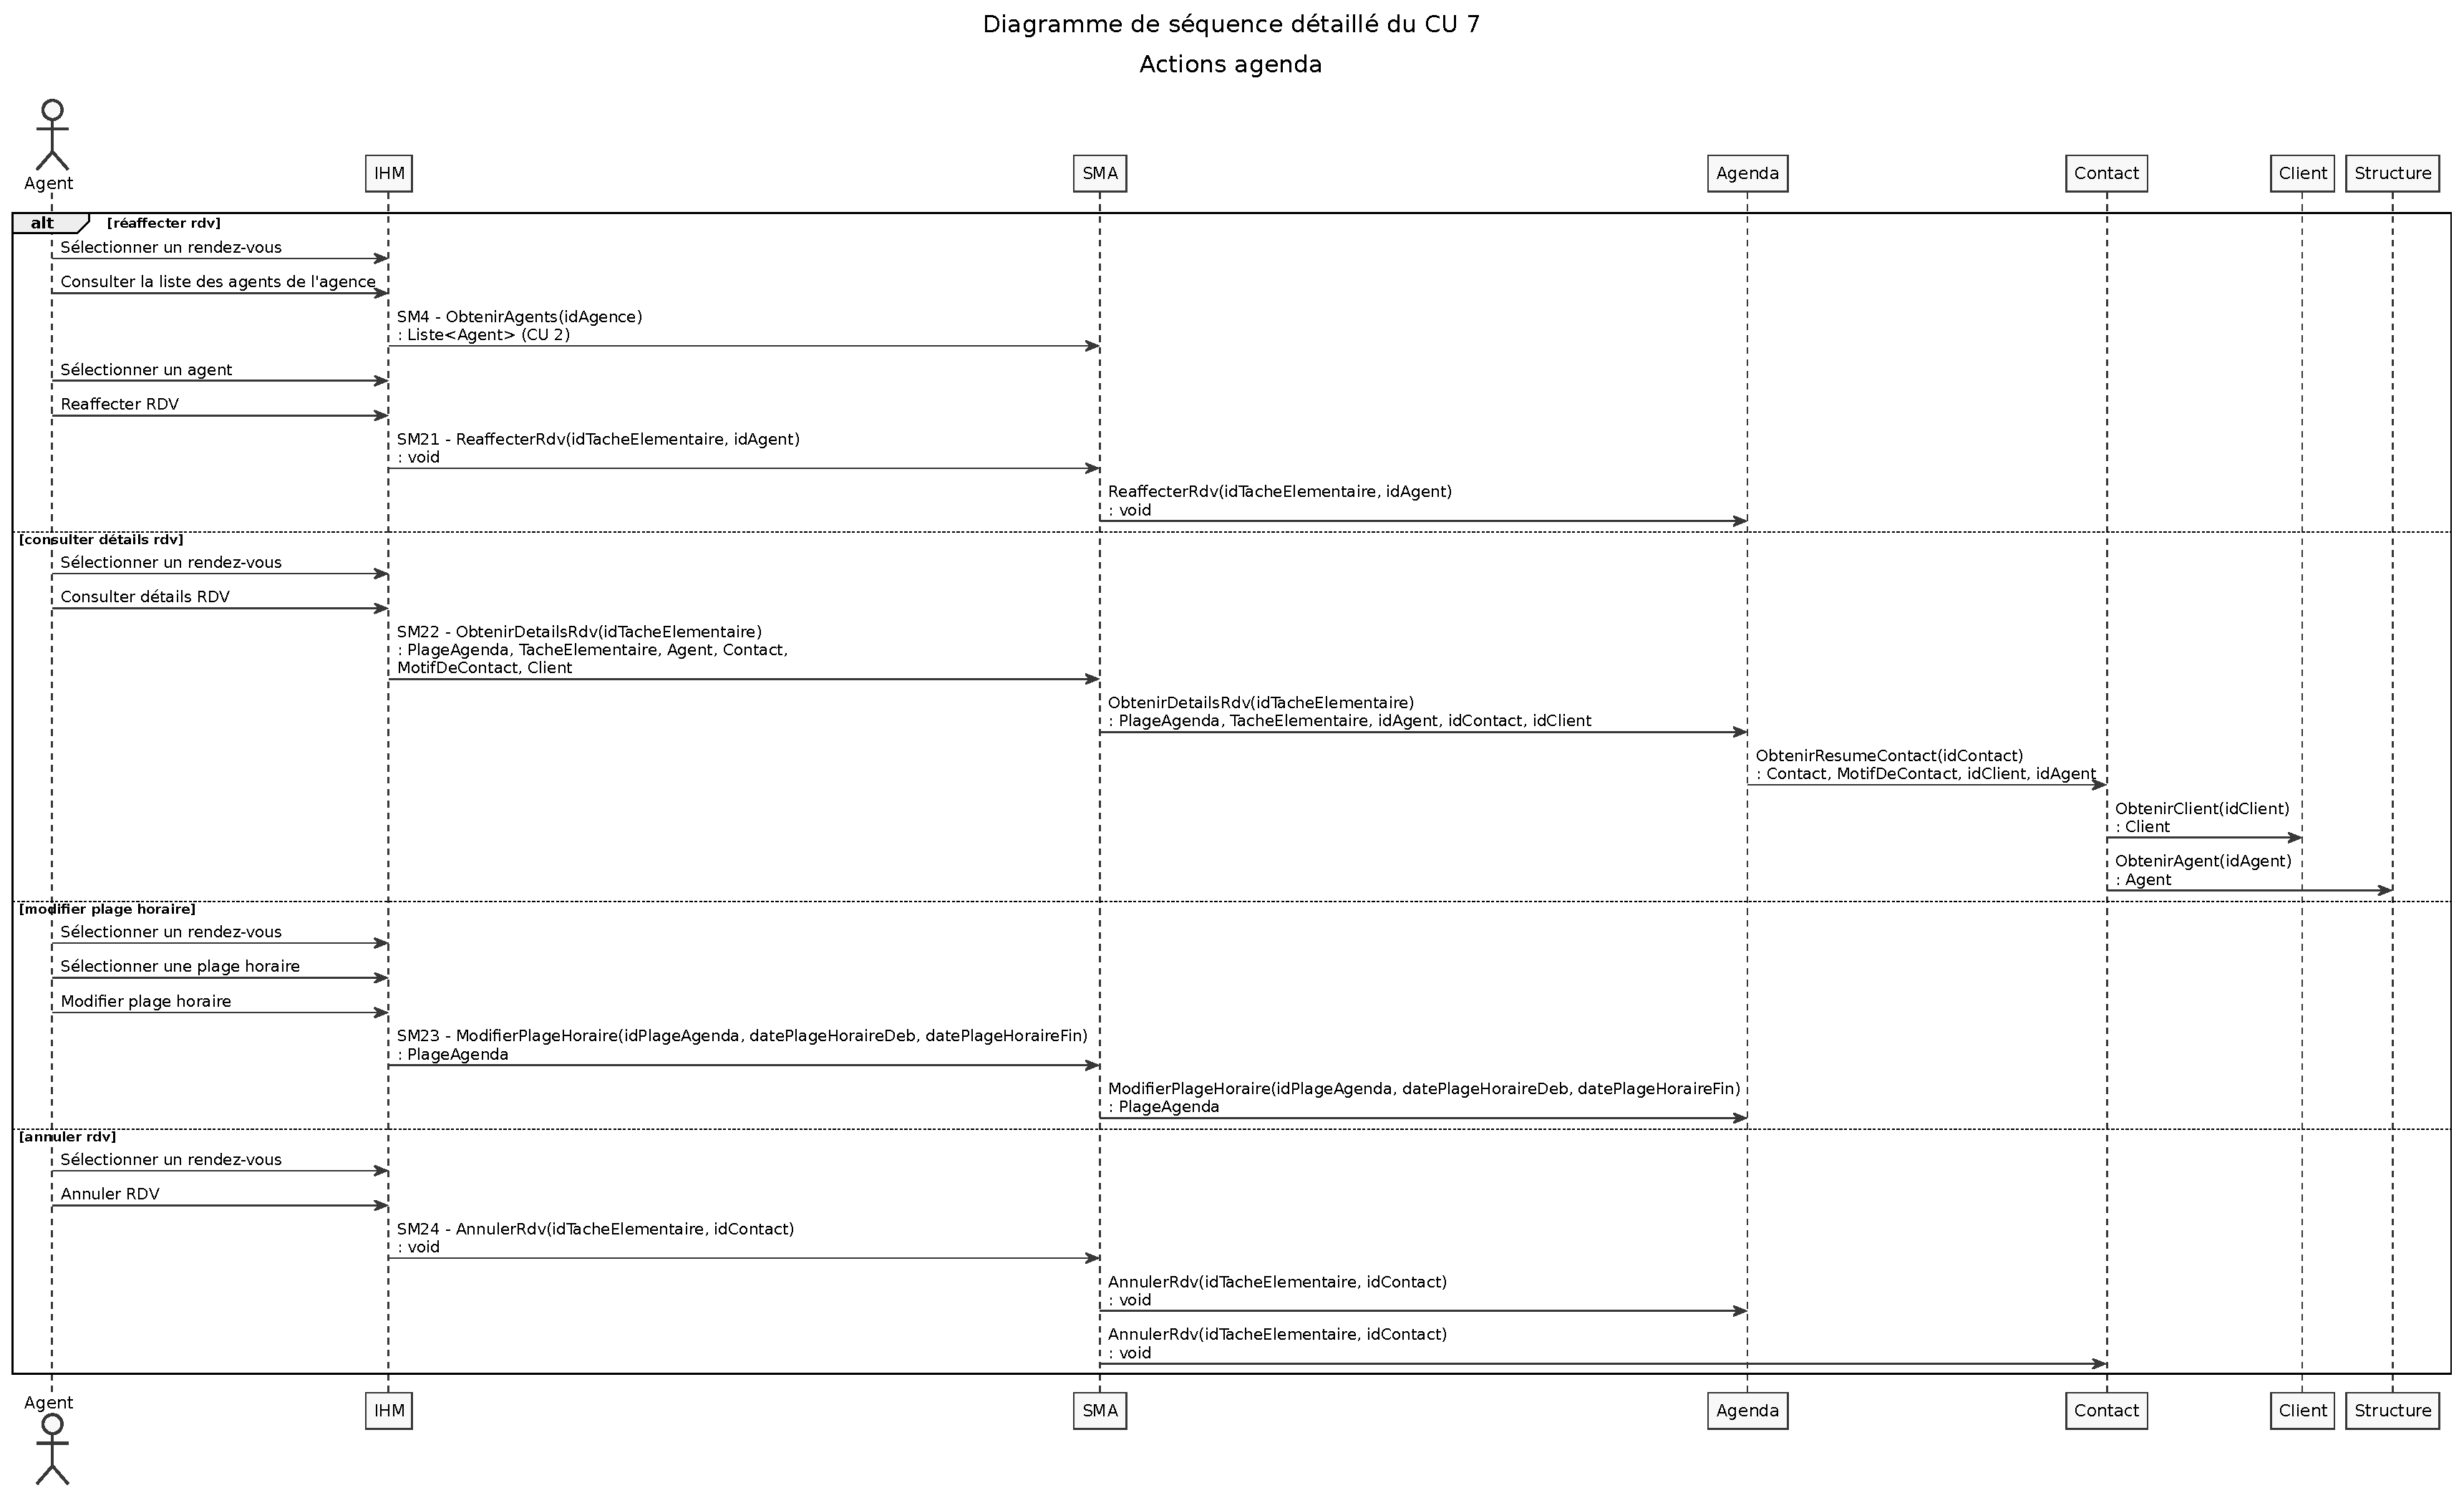
\includegraphics[height=12cm]{../report/figures/eps/DSD_CU7_ActionsAgenda}}}



    \end{frame}
    
     \begin{frame}{Diagramme de séquence détaillé - Action Agenda}
    \adjustbox{width=1.1\textwidth, center, trim={0} {0} {0} {.5\height},clip}%
  {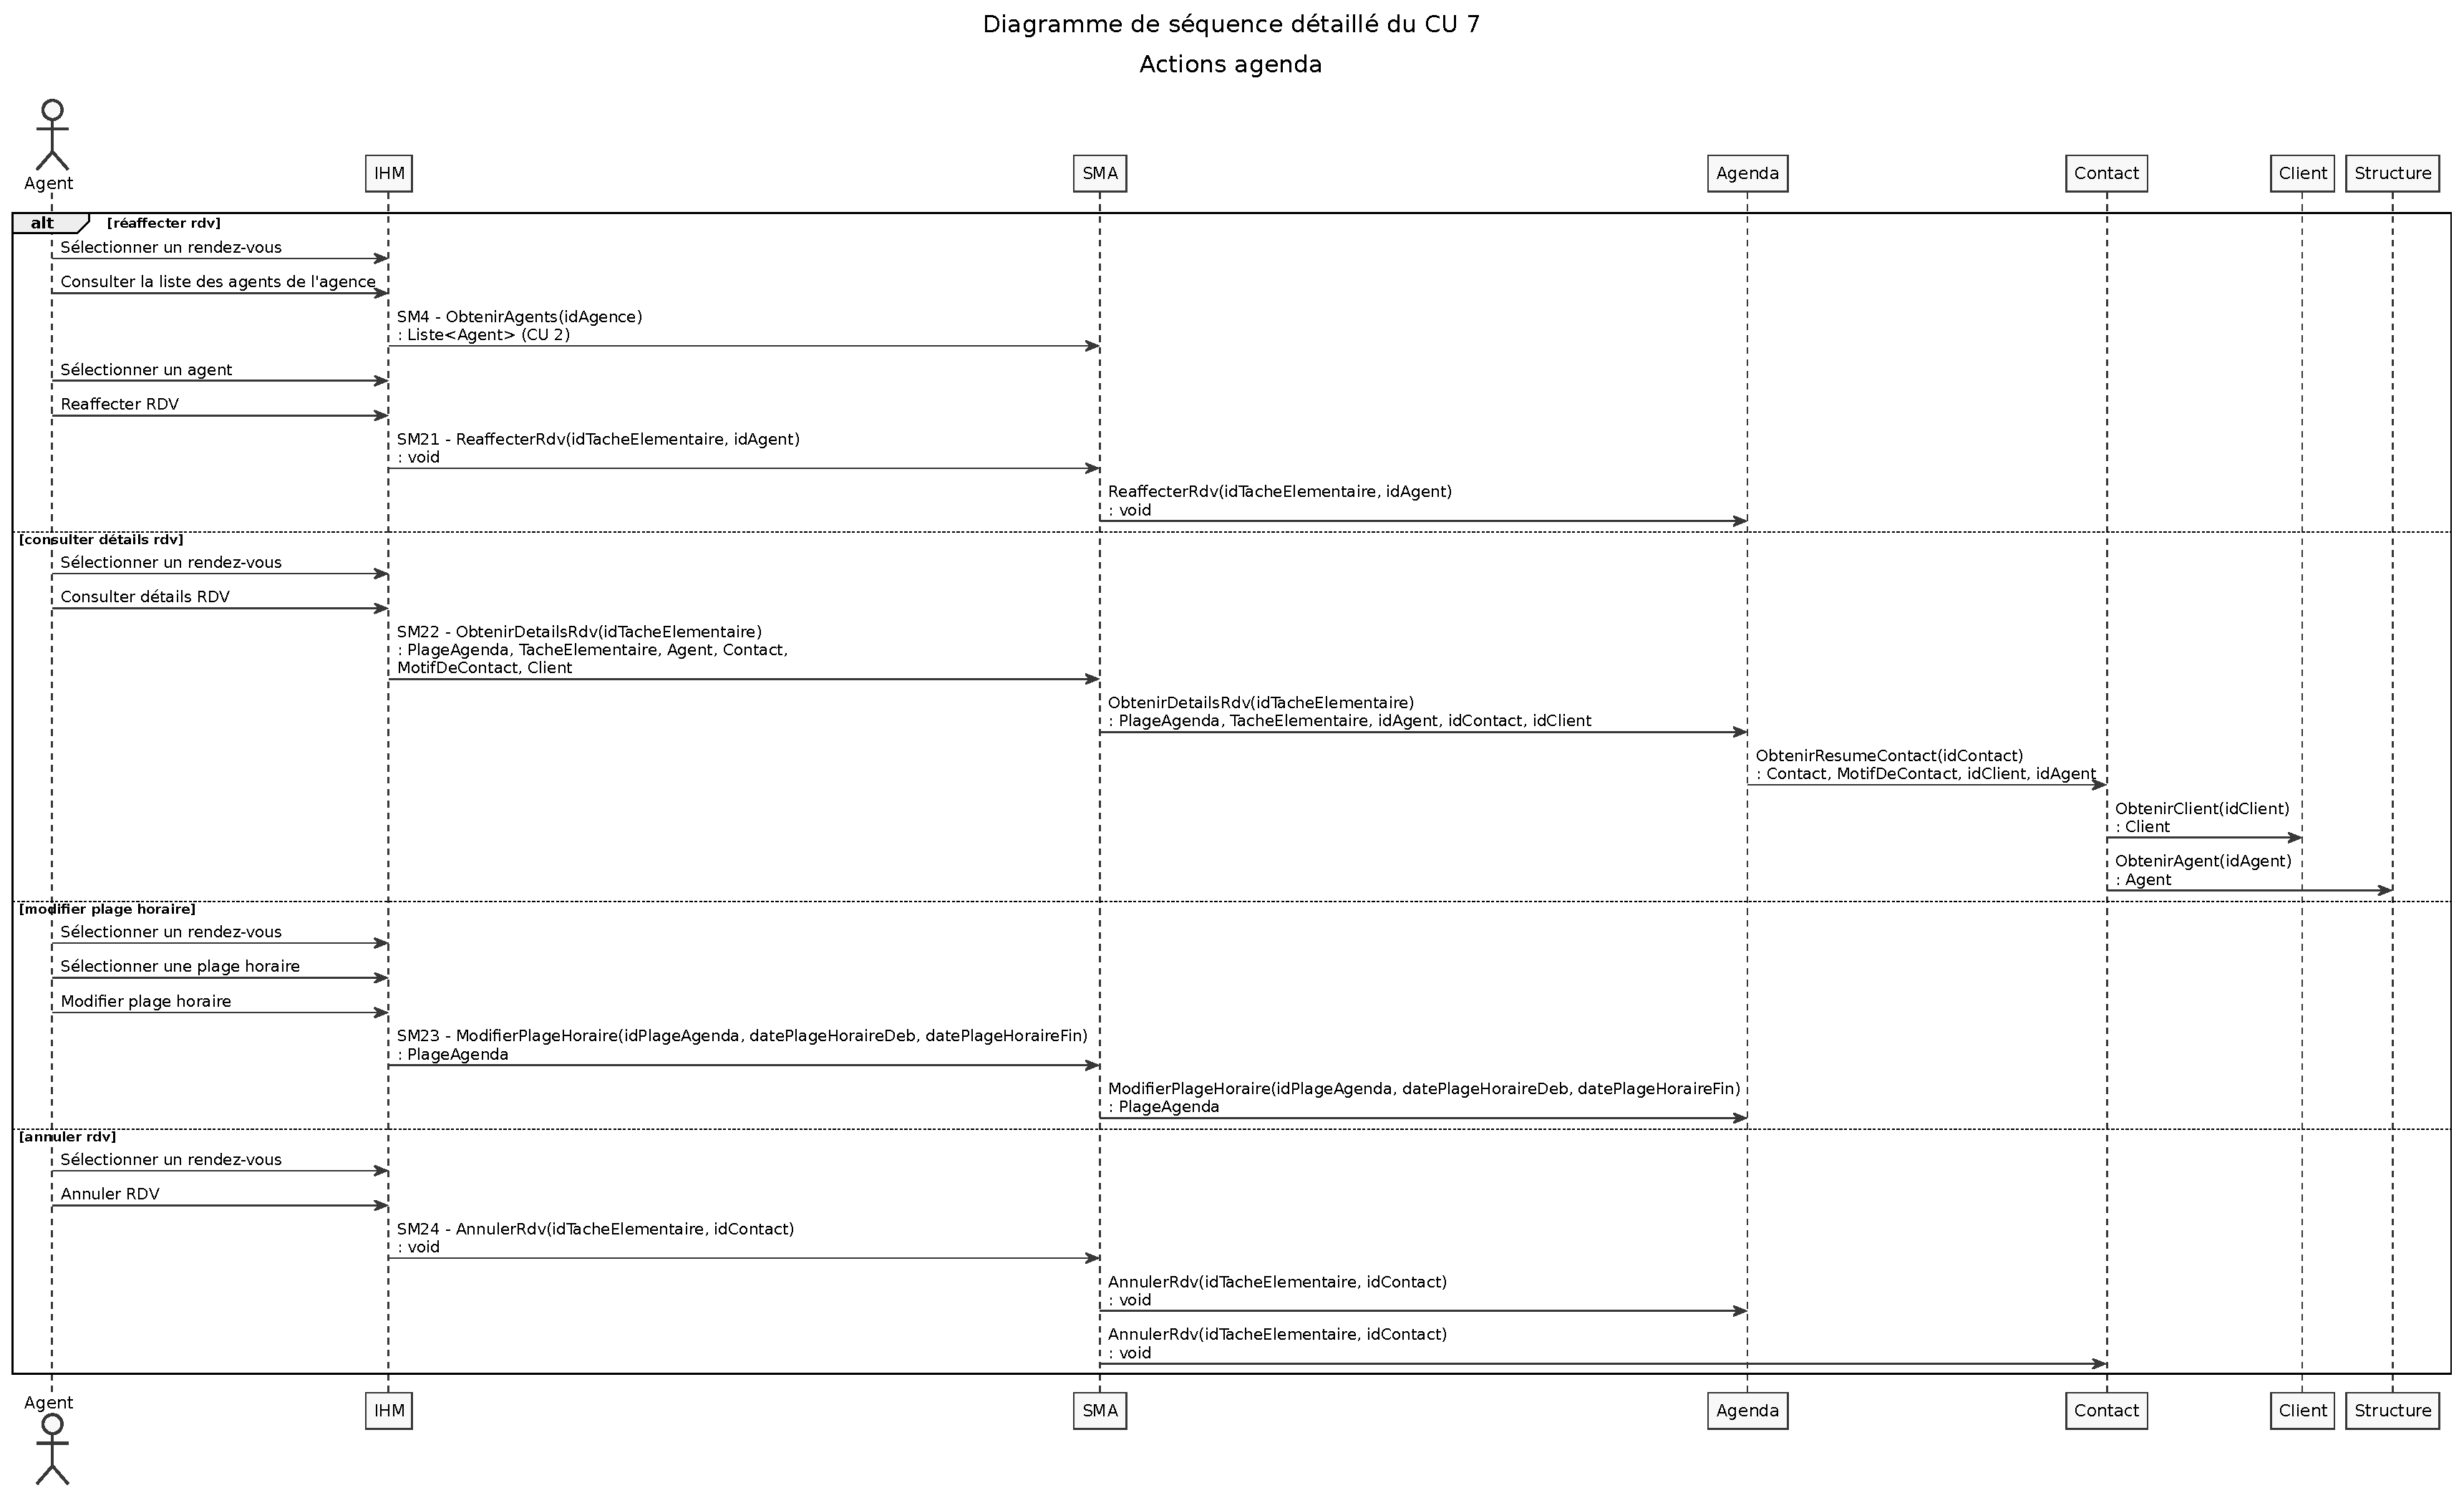
\includegraphics[height=12cm]{../report/figures/eps/DSD_CU7_ActionsAgenda}}
    \end{frame}
    
    
    \section{Diagramme de collaboration}
    \begin{frame}{Diagramme de collaboration}
\noindent\makebox[\textwidth]{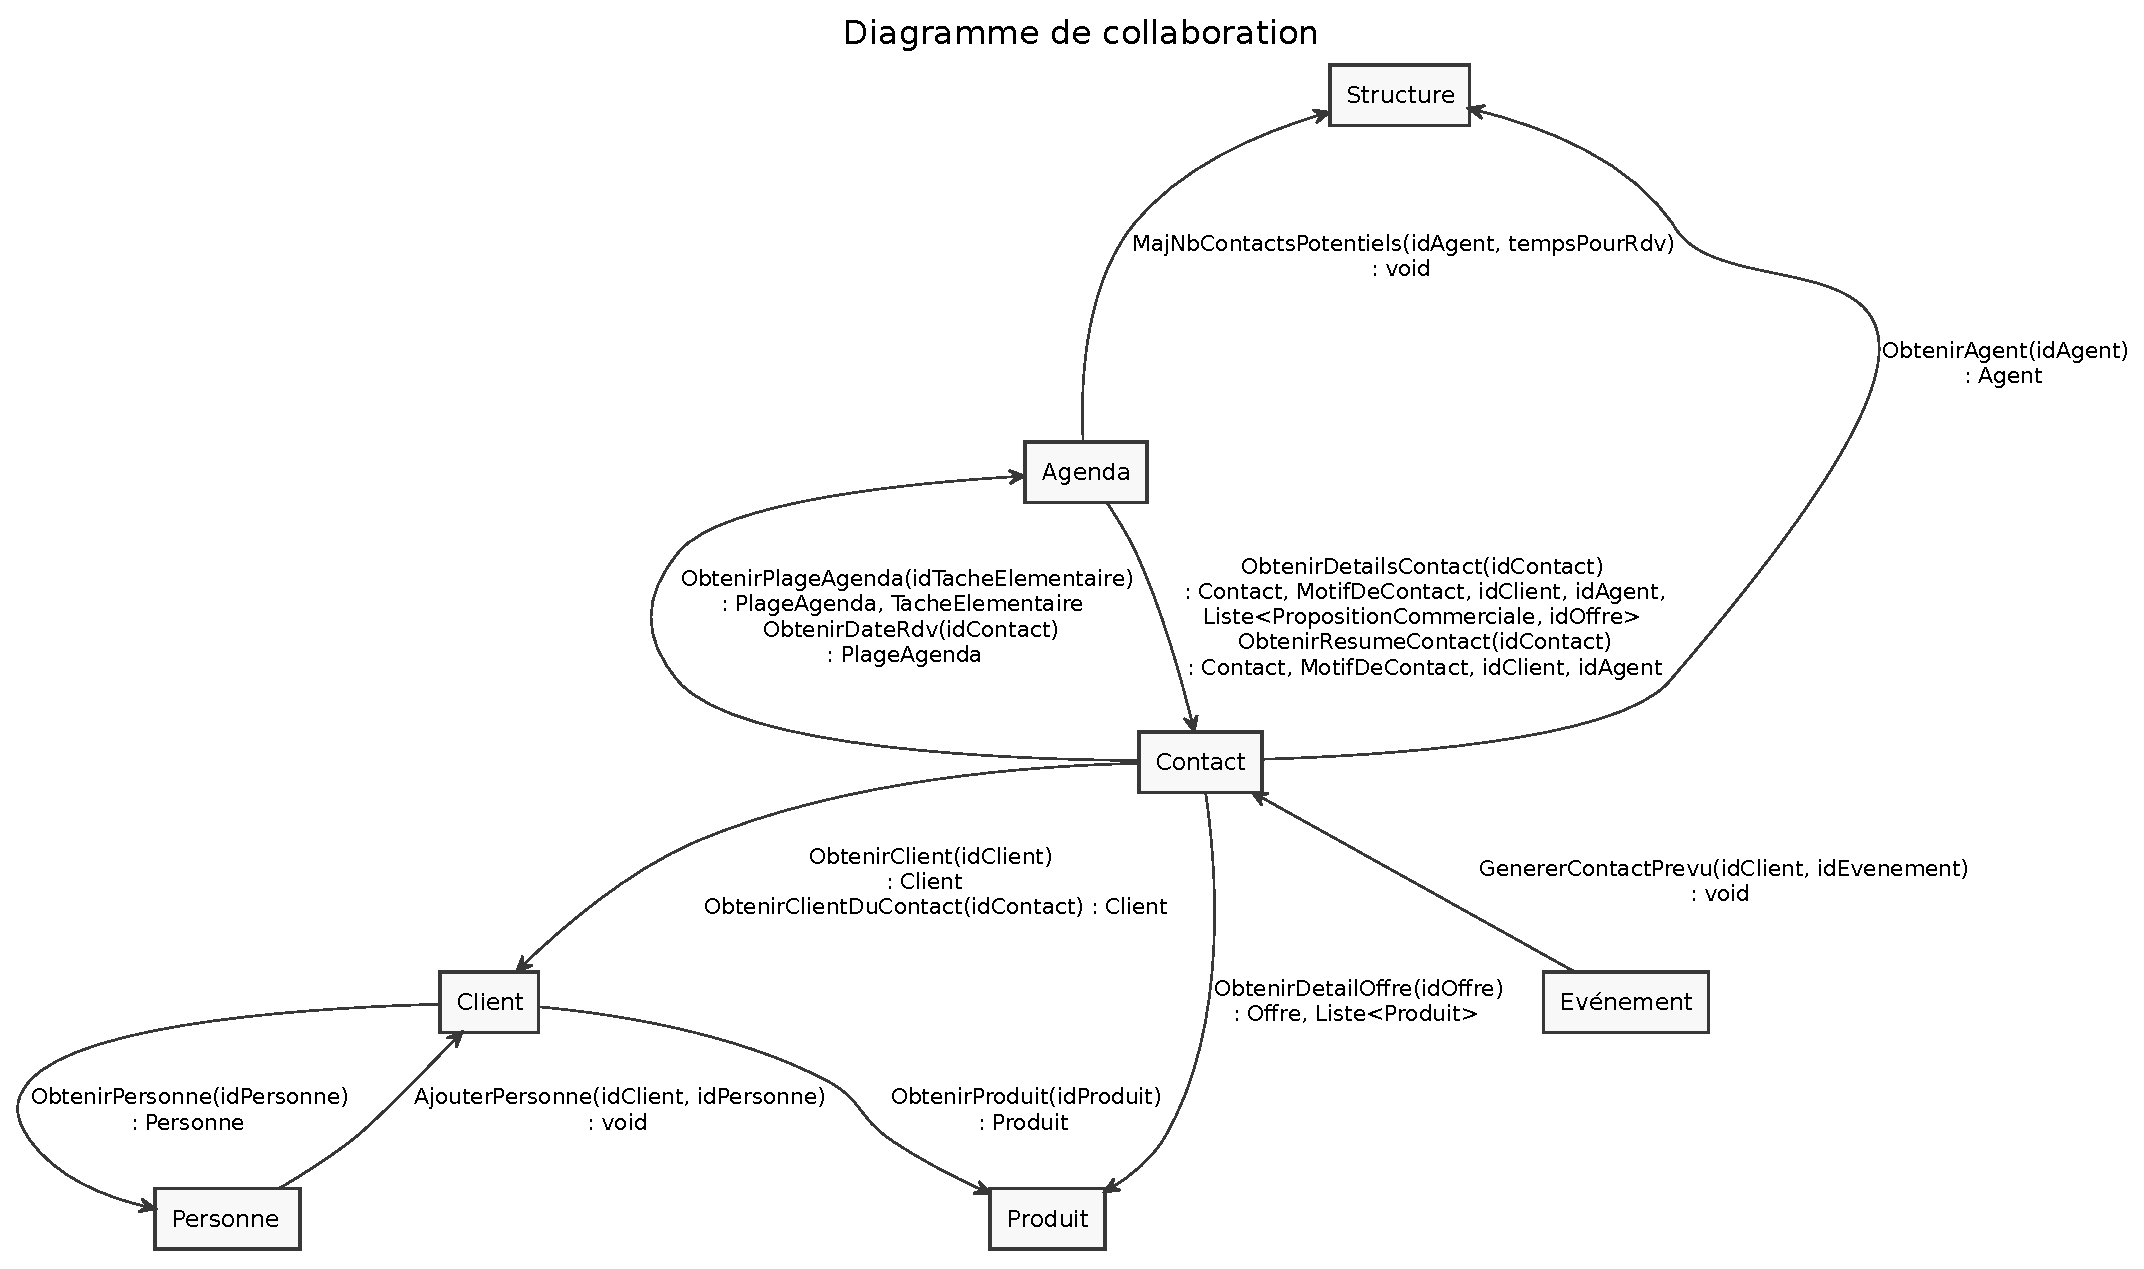
\includegraphics[height=5.5cm]{../report/figures/eps/collaboration}}
    \end{frame}
    
    \section{2 SM + SOM (Pierre)}
    \begin{frame}{SMA - Obtenir Détail Agent}
   \begin{small}
            \noindent \textit{\textit{Arguments en entrée :}}
\begin{description}
\item[idAgent] l'identifiant numérique de  l'agent pour lequel on souhaite obtenir l'agenda. 
\item[numSemaine] le numéro de la semaine à rechercher, de 1 à 52. 
\item[annee] l'année pour laquelle on souhaite obtenir l'agenda de la semaine mentionnée en second argument, sous format numérique, à quatre chiffres. \\
\end{description}

\noindent \textit{Sorties} :

\begin{description}
\item[Liste<PlageAgenda>] l'ensemble des plages agenda de l'agent ayant l'identifiant idAgent, pour la semaine numSemaine de l'année annee.
\item[Liste<TacheElementaires>] l'ensemble des tâches élémentaires associées aux plage agenda également retournées. 
\item[Liste<TypeActivite>] l'ensemble des activités de l'agent qui lui sont affectées sur les plage agenda également retournées. \\
\end{description}
   \end{small}
    \end{frame}
    \begin{frame}{SMA - Obtenir détails rdv}

\begin{small}
\noindent \textit{Arguments en entrée :}
\begin{description}
\item[idPlageAgenda] l'identifiant de la plage agenda qui représente le rendez-vous que l'on souhaite détailler. \\
\end{description}

\noindent \textit{Sorties} : 
\begin{description}
\item[PlageAgenda] la plage agenda associée à l'identifiant passé en paramètre. 
\item[Agent] l'agent associé à la plage agenda retournée et, de fait, associé au rendez-vous que l'on souhaite détailler. 
\item[Contact] le contact qui est associé à la plage agenda retournée et qui doit être (ou à été) réalisé durant ce créneau horaire.
\item[MotifDeContact] le motif du contact de la plage agenda possédant l'identifiant passé en paramètre. 
\item[Client] le client concerné par le rendez-vous. \\
\end{description}
\end{small}
    \end{frame}
    
    \begin{frame}{Bilan du projet}
  \begin{figure}
	\begin{tikzpicture}
      \begin{axis}[
        mbarplot,
        ylabel=Temps (Heures),
        axis y line=left,
        axis x line=bottom,
        xmin=0, xmax=5,
        ymin=0, ymax=40,
        xtick={1,2,3,4},
        xticklabels={Conception\\ d’ensemble,Conception\\ fonctionnelle\\ détaillée,Conception\\ applicative\\ détaillée,Architecture\\ technique},%<--Here
        xlabel style={yshift=-1cm},
        x tick label style={
            rotate=62,
            anchor=east,
            font=\footnotesize,
            align=right
        },
        width=\textwidth,
        height=7cm,
      ]

      \addplot plot coordinates {(1, 20) (2, 25) (3, 22.4) (4, 12.4)};
      \addplot plot coordinates {(1, 18) (2, 24) (3, 23.5) (4, 13.2)};

      \legend{Temps estimé, Temps passé}

      \end{axis}
    \end{tikzpicture}
  \end{figure}
\end{frame}

\end{document}
